\subsection{DAC Control} \label{subsec:DAC_CONTROL} 
Section \refq{ch:SysArchitecture} shows that the the Sample Controller is responsible for controlling the DAC such that a stable sine wave is generated. The logic responsible for this will be described in this section. The specific section of the Sample Controller that handles the DAC logic is referred to as the DAC Control. A block diagram of the DAC Control can be seen on figure \refq{fig:7_2_3_DAC_CONTROL}.

\begin{figure}[H]
    \centering
    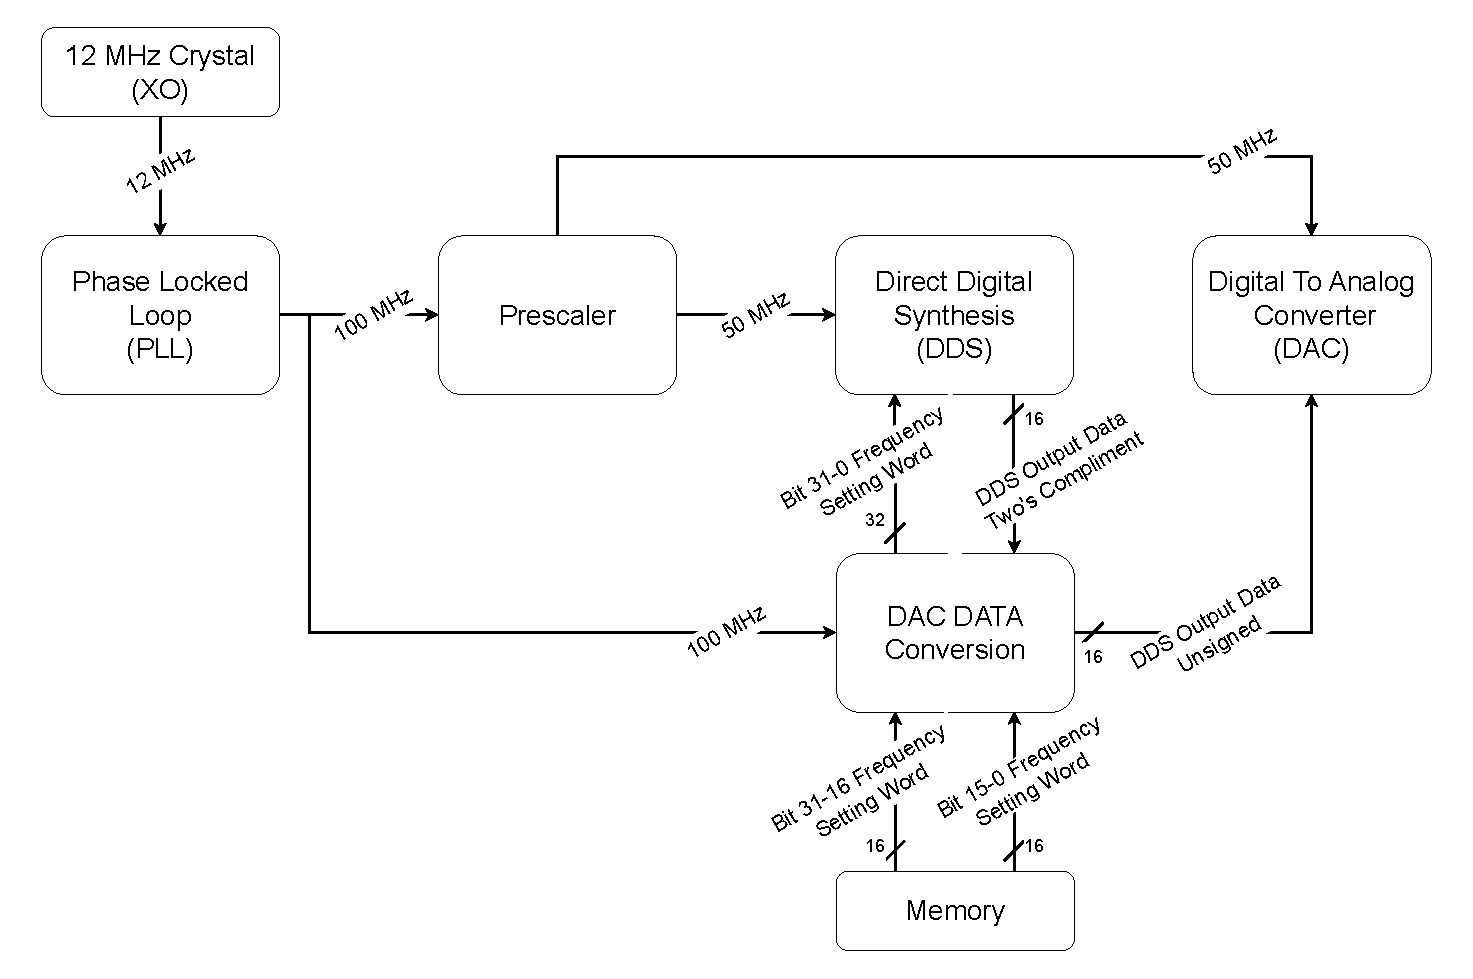
\includegraphics[clip, trim=0 0 0 0, width=1\textwidth]{Sections/7_SystemDesign/Figures/7_2_3_DAC_CONTROL.pdf}
    \caption{Block diagram of the DAC Control logic, the DAC is on the Analog Front End, it is shown here for completeness.}
    \label{fig:7_2_3_DAC_CONTROL}
\end{figure}

There are numerous of ways to generate sine waves, for this project a digital implementation has been favored due to the precise resolution that it offers. Requirement §1 from section \refq{ch:SystemRequirements} states that the frequency resolution must be at least \SIQ{1}{\hertz}. To achieve this, a Direct Digital Synthesis (DDS) principle has been implemented. This essentially allows for a frequency resolution that is the DAC update rate divided by the length of the frequency setting word \cite{Fundamentals_DDS}. With a 32 bit wide frequency setting word, as specified by requirement §6.3.13 in section \refq{subsec:SampleControlSpec}, the resulting frequency resolution would be $f_{res} = \frac{DAC_{CLK}}{2^{32}}$.

The used DAC is an LTC1668, capable of an update rate of \SIQ{50}{\mega\hertz}, it has however been decided to use \SIQ{20}{\mega\hertz} as \SIQ{50}{\mega\hertz} square waves are rather difficult to handle on development boards. This essentially allows for a frequency resolution of \SIQ{4.6566}{\milli\hertz}, see equation \refq{eq:7_2_3_resolution}, assuming an update rate of \SIQ{20}{\mega\hertz}.

\begin{equation}
    \label{eq:7_2_3_resolution}
    f_{res} = \frac{\SIQ{20}{\mega\hertz}}{2^{32}} \Rightarrow \SIQ{4.6566}{\milli\hertz}. 
\end{equation}

Xilinx offers a complete "drag and drop" DDS block. The project team has settled on using this as it supports DAC resolutions of up to 26 bits and frequency setting words up to 48 bits, essentially making it ideal for the required DAC Control block. The principle of Direct Digital Synthesis will not be explained in this document, as it is not part of the scope of the project.

The DDS block is configured to take in a 32 bit wide frequency setting word, a \SIQ{20}{\mega\hertz} clock, and a frequency update signal. The output of the DDS block is configured for a 16 bit wide sine approximation as two's compliment.

All other blocks than the DDS shown in figure \refq{fig:7_2_3_DAC_CONTROL} are essentially there to "support" the DDS block. A \SIQ{20}{\mega\hertz} clock is generated via a Phase Locked Loop (PLL) and a prescaler. The PLL outputs a \SIQ{200}{\mega\hertz} signal that is divided by ten and fed to the DDS block. The prescaler will also generate a \SIQ{20}{\mega\hertz} pulse train that is delayed from the DDS clock signal. This delayed pulse train is used to update the DAC and to detect if a new frequency setting word is present. The PLL is an integrated solution from Xilinx, much like the DDS block, and as such it will not be explained further.

The 16 bit wide output data of the DDS contains an approximated full-scale sine wave in two's compliment. The DAC however requires unsigned values as an input, and thus the DDS output data must be converted to a 16 bit wide unsigned bus. Furthermore the memory holds data in 16 bit registers, meaning that the 32 bit frequency setting word must be two registers that are concatenated. The DAC DATA Conversion block handles this concatenation and conversion from two's compliment to unsigned.

\subsubsection{DDS and DAC Prescaler}
The clock for the DDS and DAC are both derived from the \SIQ{200}{\mega\hertz} master clock. This clock is divided down to a \SIQ{20}{\mega\hertz} clock by the use of a counter and a D flip flop. This can be seen in listing \ref{lst:7_2_3_DAC_Prescaler}. 

\lstinputlisting[language=c ,style = c,firstnumber=1, linerange=34-63, caption={Code for DDS and DAC prescaler}, label={lst:7_2_3_DAC_Prescaler}]{Sections/7_SystemDesign/Code/DAC_PRESCALER.vhd}

When a rising edge of the master clock occurs on i\_CLK the counter will increment by one. Once the counter has incremented to 4, the 5th.ed. clock will reset the counter and togle the output. Thus the system can be seen as a counter that resets the counter on the 5th clock. One thing to keep in mind when using HDL, is that it is not code, but the behaviour of hardware that is described. To show the intention of the HDL code in listing \ref{lst:7_2_3_DAC_Prescaler}, figure \ref{fig:7_2_3_DAC_PRESCALER_LOGIC} can be used. Here a 3 bit counter is designed by the use of D flip flops, when the value 5 is present on the output of the coutner, it resets itself. This reset pulse then drives another D flip flop. The counter divides by 5, and the final flip flop by 2, resulting in the master clock being divided by 10. The reset pulse of the counter is very short, it goes high, and as a result it practically instantly goes low again due to the coutner reseting itself. It is generaly not desireable to have such a short pulse as a clock signal, hence the final flip flop. This flip flop will ensure a \SIQ{50}{\%} duty cycle of the output clock.

\begin{figure}[H]
    \centering
    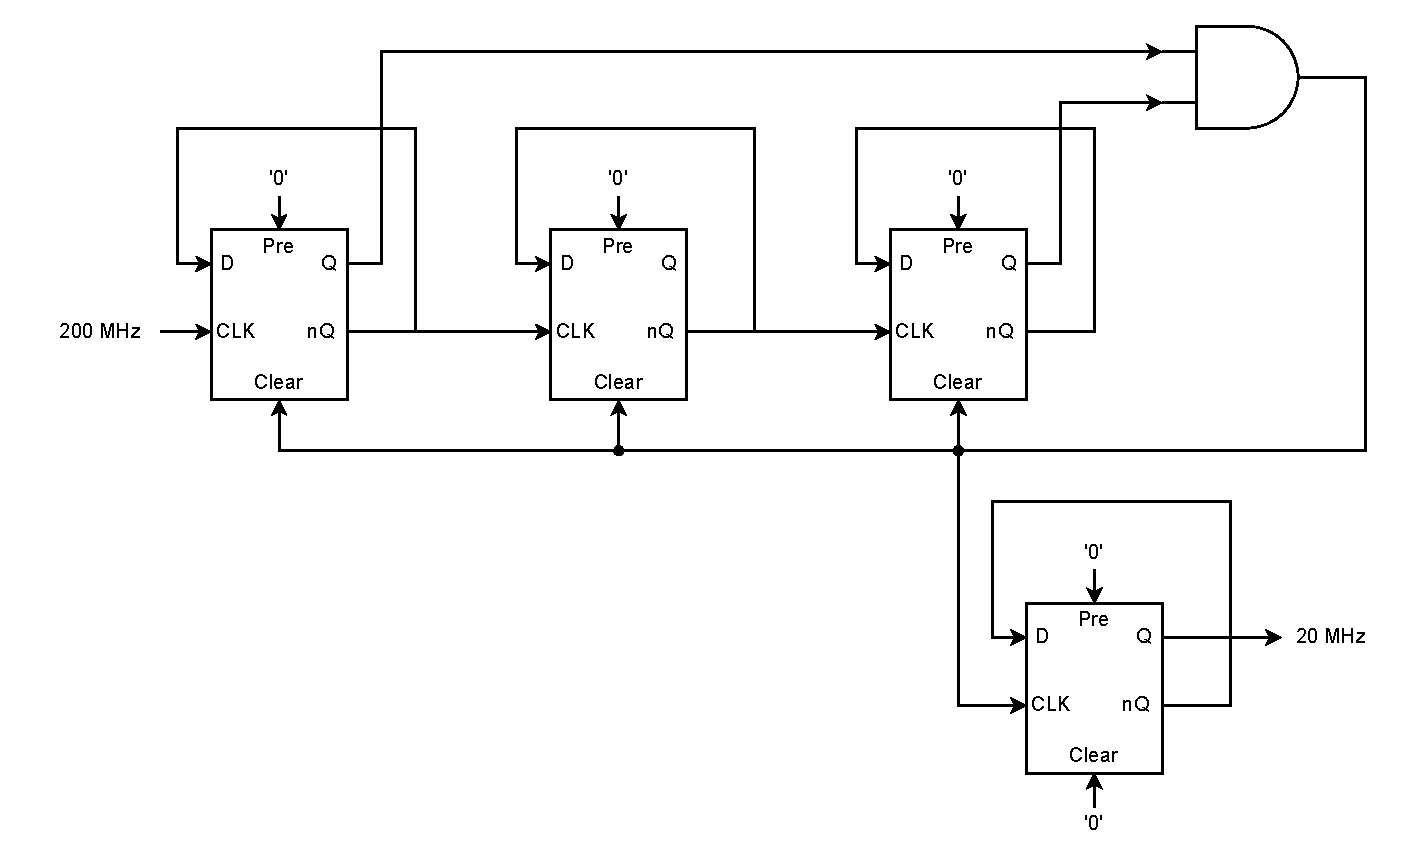
\includegraphics[clip, trim=0 0 0 0, width=1\textwidth]{Sections/7_SystemDesign/Figures/DAC_PRESCALER_LOGIC.pdf}
    \caption{Logic diagram of the DAC prescaler.}
    \label{fig:7_2_3_DAC_PRESCALER_LOGIC}
\end{figure}


The DAC and DDS must be updated not exactly at the same time. This is crucial, as the DAC will update its output to the code present on its data inputs on a rising edge of its clock. The DDS will likewise update its output code on the same edge if they are updated by the same clock. To avoid this, the DAC is clocked by the inverse DDS clock. Thus the DAC is updated \SIQ{180}{\degree} out of phase from the DDS. This will have allowed the DDS data to have settled before the DAC uses it to update its output. A diagram of these signals can be seen in figure \ref{fig:7_2_3_DAC_PRESCALER}.

\begin{figure}[H]
    \centering
    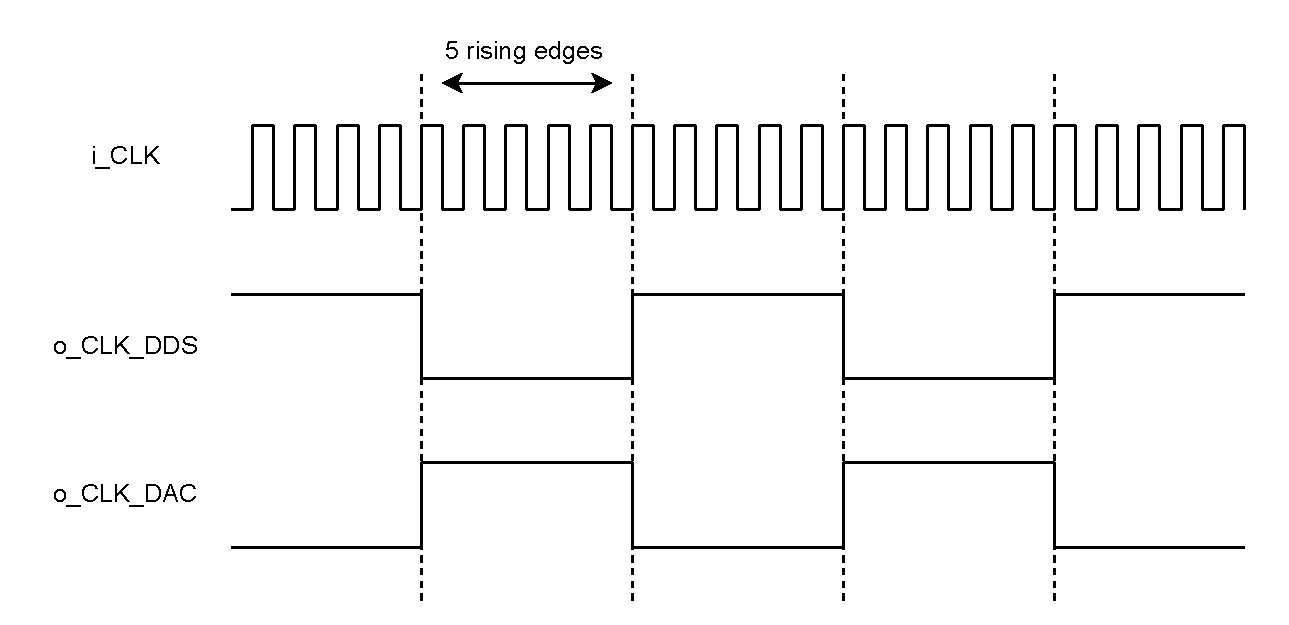
\includegraphics[clip, trim=0 0 0 0, width=1\textwidth]{Sections/7_SystemDesign/Figures/DAC_PRESCALER.pdf}
    \caption{Timing diagram of the input clock and output signals of the DDS and DAC Prescaler.}
    \label{fig:7_2_3_DAC_PRESCALER}
\end{figure}

\subsubsection{DAC DATA Conversion}
The DAC DATA Conversion block ensures that the DAC is fed appropriate data and that the DDS block receives the proper 32 bit wide frequency setting word, as well as indicating to the DDS that new data is available for the frequency setting. The VHDL code for the DAC DATA Conversion can be seen in listing \refq{lst:7_2_3_DAC_DATA_Conversion}.

\lstinputlisting[language=c ,style = c,firstnumber=1, linerange=34-70, caption={Code for DAC DATA Conversion}, label={lst:7_2_3_DAC_DATA_Conversion}]{Sections/7_SystemDesign/Code/DAC_DATA_Conversion.vhd}

Lines 3 through 5 in listing \refq{lst:7_2_3_DAC_DATA_Conversion}, shows that it takes in i\_LoByte\_FWORD and i\_LoByte\_FWORD, and puts out o\_FWORD, byte is a bit misleading here as they are 16 bit values. The two inputs are both 16 bit wide busses and the output o\_FWORD is a 32 bit wide bus. Line 21 in the same list shows how the two inputs, i\_HiByte\_FWORD and i\_LoByte\_FWORD, are concatenated to form the 32 bit output bus o\_FWORD.

The DAC DATA Conversion also takes in i\_DDS\_DATA and outputs o\_DAC\_DATA, line 7 and 8 in list \refq{lst:7_2_3_DAC_DATA_Conversion}. Line 24 shows that o\_DAC\_DATA is rather simply i\_DDS\_DATA xor'ed with the hex value "8000" or rather 32768 in decimal. This is the MSB value, and it results in the two's compliment data from the DDS being converted to unsigned values.

To see the effect of xor'ing two's compliment with the MSB, an example of the same operation with a 3 bit variable is shown in table \refq{tab:7_2_3_DAC_DATA_Conversion}. Here it can be seen that the result is that all values are offset by the value of the MSB, in the case of a 3 bit variable, it results in all values being offset by 4, or all values are added a value of 4. 

This is exactly what is desired, as the DAC output should be centered around an offset value, as the DAC cannot output negative values.

\begin{table}[H]
    \begin{tabular}{|l|l|l|l|}
    \hline
    \begin{tabular}[c]{@{}l@{}}A\\ Decimal\end{tabular} & \begin{tabular}[c]{@{}l@{}}A\\ 2's Comp\end{tabular} & B = A xor 100 & \begin{tabular}[c]{@{}l@{}}B\\ Decimal\end{tabular} \\ \hline
    3                                                   & 011                                                  & 111       & 7                                                           \\ \hline
    2                                                   & 010                                                  & 110       & 6                                                           \\ \hline
    1                                                   & 001                                                  & 101       & 5                                                           \\ \hline
    0                                                   & 000                                                  & 100       & 4                                                           \\ \hline
    -1                                                  & 111                                                  & 011       & 3                                                           \\ \hline
    -2                                                  & 110                                                  & 010       & 2                                                           \\ \hline
    -3                                                  & 101                                                  & 001       & 1                                                           \\ \hline
    -4                                                  & 100                                                  & 000       & 0                                                           \\ \hline
    \end{tabular}
    \caption{Example of two's compliment, A, xor'ed with the MSB of a 3 bit integer. The result is in the form of an unsigned integer
    0 having been offset by the value of the MSB.}
    \label{tab:7_2_3_DAC_DATA_Conversion}
    \end{table}

    The process in line 27 trough 37 in listing \refq{lst:7_2_3_DAC_DATA_Conversion} shows how the logic detects if the frequency setting words has been updated. When a rising edge of the i\_CLK here the same clock that drives the DAC, takes place, the input data r\_F\_IN and latched output data r\_F\_OUT are compared, if they are not the same, the logic will set w\_update\_F to high, and update the latched output data to match the input data. On the next rising edge of i\_CLK, the data will be the same, and here w\_update\_F is then set to low again. This creates a pulse the length of the period of i\_CLK, only when new data is present on r\_F\_IN. 
    
    The DDS block will update its output frequency when a rising edge appears on its update frequency input, and thus the DDS will only update its output frequency when new data is present on r\_F\_IN, and r\_F\_IN is generated from concatenating the two memory registers containing the DAC frequency, resulting in the DDS only updating its frequency when the MCU programs in a new frequency to the memory.